\documentclass[11pt,compress,t,notes=noshow, aspectratio=169, xcolor=table]{beamer}

\usepackage{../../style/lmu-lecture}
% Defines macros and environments
% This file is included in slides and exercises

% Rarely used fontstyle for R packages, used only in 
% - forests/slides-forests-benchmark.tex
% - exercises/single-exercises/methods_l_1.Rnw
% - slides/cart/attic/slides_extra_trees.Rnw
\newcommand{\pkg}[1]{{\fontseries{b}\selectfont #1}}

% Spacing helpers, used often (mostly in exercises for \dlz)
\newcommand{\lz}{\vspace{0.5cm}} % vertical space (used often in slides)
\newcommand{\dlz}{\vspace{1cm}}  % double vertical space (used often in exercises, never in slides)
\newcommand{\oneliner}[1] % Oneliner for important statements, used e.g. in iml, algods
{\begin{block}{}\begin{center}\begin{Large}#1\end{Large}\end{center}\end{block}}

% Don't know if this is used or needed, remove?
% textcolor that works in mathmode
% https://tex.stackexchange.com/a/261480
% Used e.g. in forests/slides-forests-bagging.tex
% [...] \textcolor{blue}{\tfrac{1}{M}\sum^M_{m} [...]
% \makeatletter
% \renewcommand*{\@textcolor}[3]{%
%   \protect\leavevmode
%   \begingroup
%     \color#1{#2}#3%
%   \endgroup
% }
% \makeatother


\tikzset{main node/.style={rectangle,draw,minimum size=1cm,inner sep=4pt},}

\title{Interpretable Machine Learning}
% \author{LMU}
%\institute{\href{https://compstat-lmu.github.io/lecture_iml/}{compstat-lmu.github.io/lecture\_iml}}
\date{}

\def\firstrowcolor{}
\def\secondrowcolor{}
\def\thirdrowcolor{}
\def\fourthrowcolor{}

\usepackage{tikz}

\begin{document}

\newcommand{\titlefigure}{figure/ebm.jpg}
\newcommand{\learninggoals}{
% \item Model-based boosting with simple base learners
% \item Feature effect and importance in model-based boosting}
\item Motivation from GAM
\item Intelligible GAM
\item Accurate GAM + Pairwise Interactions
\item FAST feature interaction detection}

\lecturechapter{Explainable Boosting Machines}
\lecture{Interpretable Machine Learning}

\begin{frame}{Generalized Additive Models}
\textbf{Recall idea of GAMs}: $$g(\E (y_i \mid \mathbf{x}_i)) = \theta_0 + f_1(x_{i1}) + f_2(x_{i2}) + \ldots + f_p(x_{ip}),\quad i=1,\cdots, N$$
\begin{itemize}
    \item One shape function (spline) $f_j$ for each feature $\leadsto$ Intelligible    
    \item Including non-linear effects
    \item Better than GLMs in accuracy
    \item \textbf{Explainable Boosting Machines} $\leftarrow$ GAM + Gradient Boosting + Tree ensembles \citebutton{Lou et al. 2012}{https://www.cs.cornell.edu/~yinlou/papers/lou-kdd12.pdf}\\$\leadsto$ More intelligible than unrestricted full complexity models (e.g. random forest) + High accuracy close to unrestricted full complexity models
\end{itemize}
\end{frame}

\begin{frame}{Intelligible GAM - Algorithm Sketch - Part I}

\begin{figure}
    \centering
    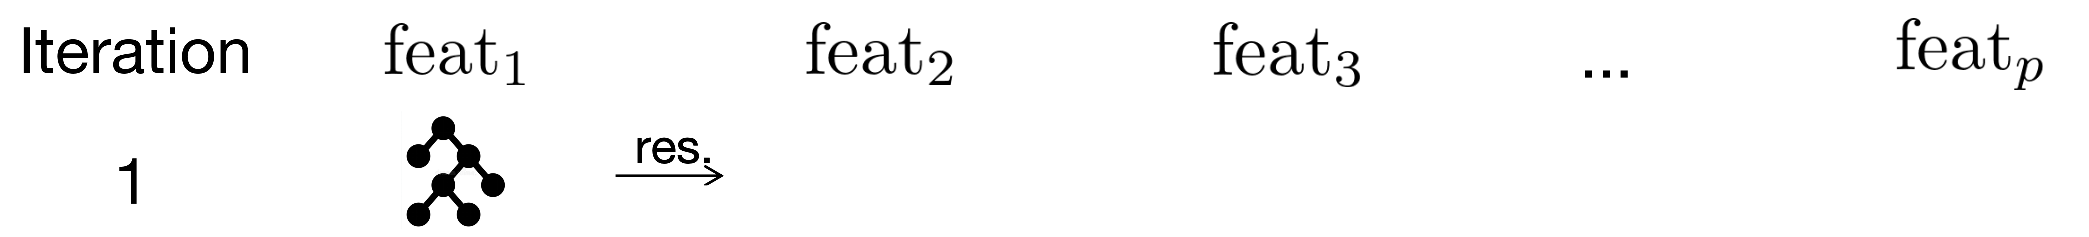
\includegraphics[width=1\linewidth]{figure/EBM_Step1.png}
    \label{fig:Intelligible EBM_Step1}
\end{figure}
\begin{itemize}
    \item Set all shape functions $f_j^{(0)}$ to zero, $j=1,\cdots,p$
    \item Calculate the initial pseudo-residual (i.e. the negative gradient of the loss function w.r.t. the current model prediction), e.g.\\
    1. for squared error loss: $\tilde{r}_i^{(0)}=-\frac{\partial L}{\partial \hat{y}_i}=y_i-\hat{y}_i^{(0)}=y_i-\sum_jf_j^{(0)}(x_{ij})$\\
    2. for log loss: $\tilde{r}_i^{(0)}=-\frac{\partial L}{\partial \hat{y}_i}=y_i-\sigma(\hat{y}_i^{(0)})$ with $\sigma(\cdot)$ being the sigmoid function
    \item Fit a shallow bagging tree with 2-4 leaves $S_1^{(1)}: x_{i1}\to \tilde{r}_i$ \textbf{only using the first feature} to predict the pseudo-residuals, with $\{x_{i1},\tilde{r}_i\}_1^N$ as training dataset
    \item Update $f_1$: $f_1^{(1)}(x_{i1})=f_1^{(0)}+\eta\cdot S_1^{(1)}(x_{i1})$
    \item Update $\hat{y}_i$: $\hat{y}_i^{(1)}=\sum_jf_j^{(1)}(x_{ij})$
    \item Update the residual w.r.t. the original target, e.g. $\tilde{r}_i^{(1)}=y_i-\hat{y}_i^{(1)}$
    \item Go to the second feature
\end{itemize}
\end{frame}

\begin{frame}{Intelligible GAM - Algorithm Sketch - Part II}
\begin{figure}
    \centering
    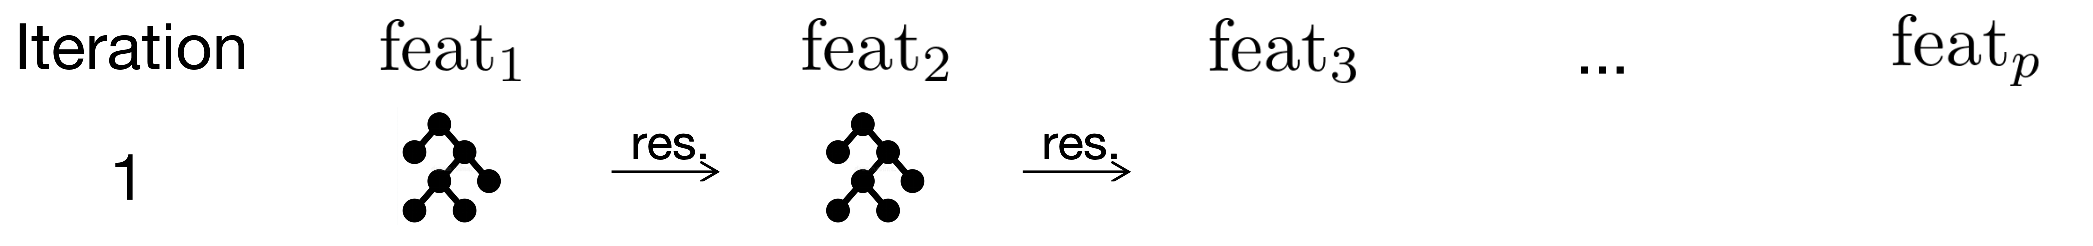
\includegraphics[width=1\linewidth]{figure/EBM_Step2.png}
    \label{fig:Intelligible EBM_Step2}
\end{figure}
\begin{itemize}
    \item Fit a shallow bagging tree $S_2^{(1)}$ \textbf{only using the second feature} to predict the updated residuals
    \item Update $f_2$ with $f_2^{(1)}(x_{i2})=f_2^{(0)}+\eta\cdot S_2^{(1)}(x_{i2})$ and then update $\hat{y}_i^{(1)}$
    \item Update the residual: this residual takes into account both what was learned on the first tree and second tree for the first two features
    \item Go to $\text{feat}_3$
\end{itemize}

\end{frame}

\begin{frame}{Intelligible GAM - Algorithm Sketch - Part III}
\begin{figure}
    \centering
    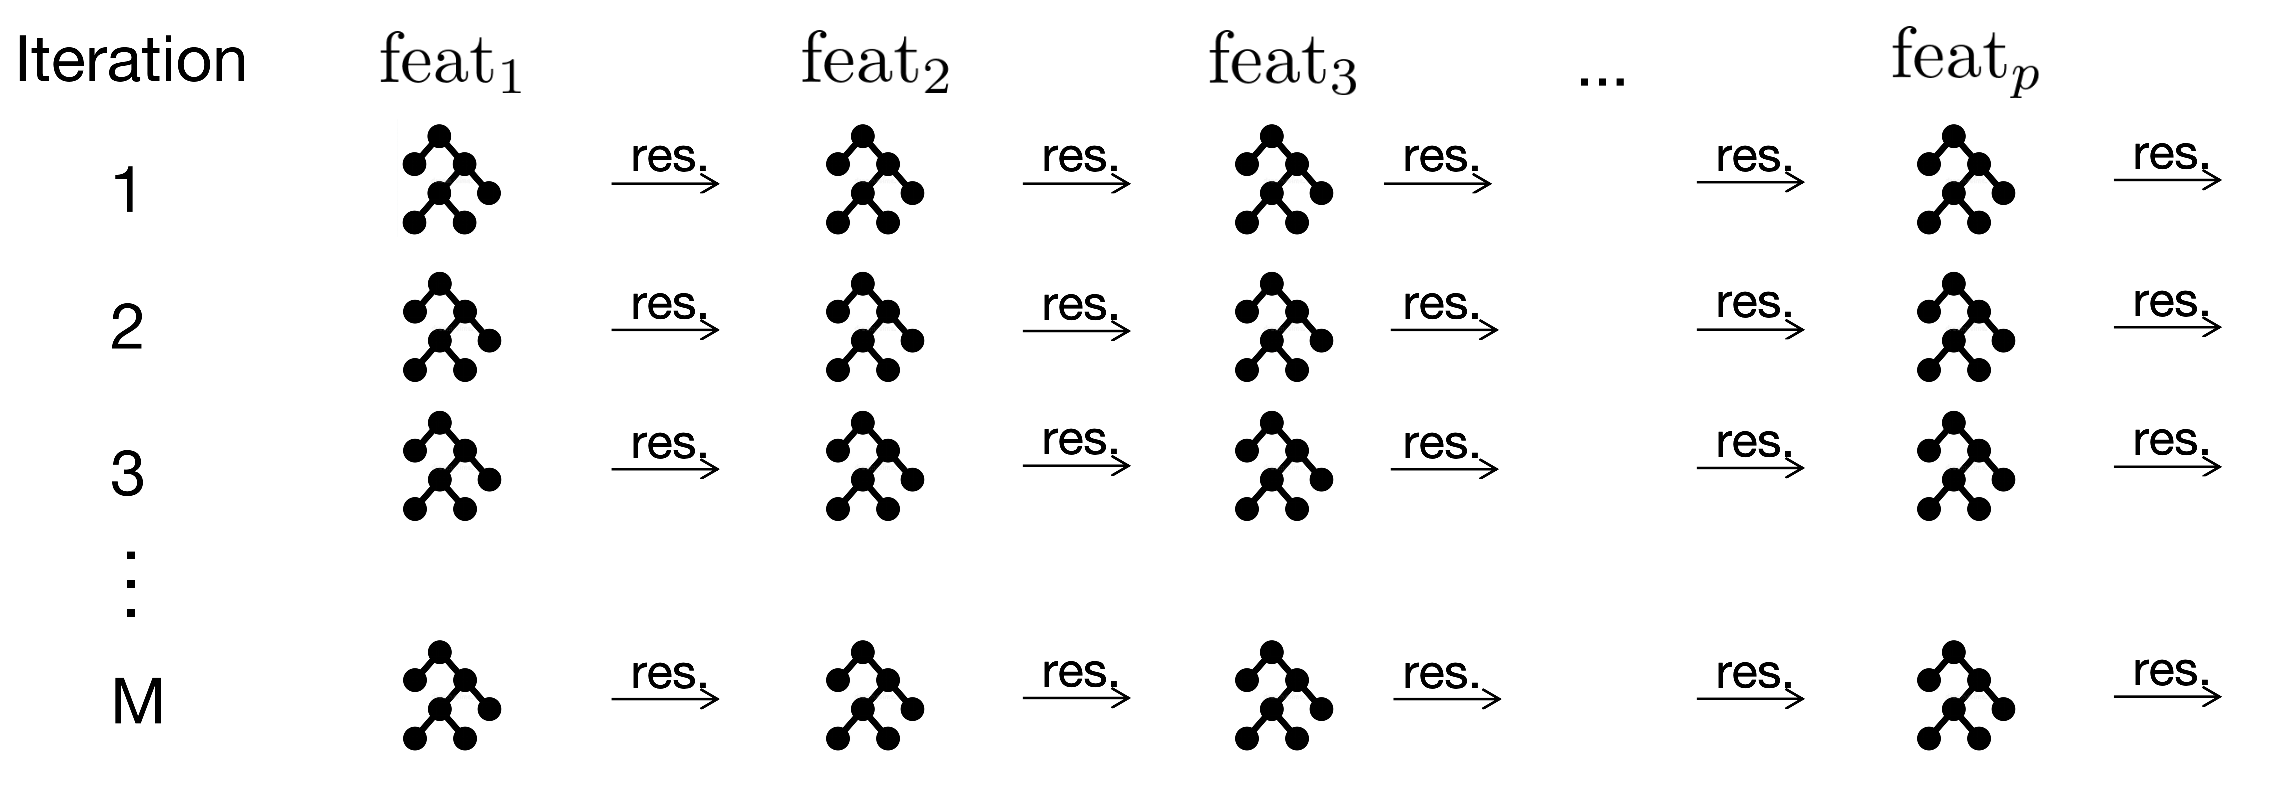
\includegraphics[width=1\linewidth]{figure/EBM_Step3.png}
    \label{fig:Intelligible EBM_Step3}
\end{figure}
\begin{itemize}
    \item Go through every feature and keep updating the residual
    \item Grow a small tree on each feature but just one at a time in each iteration
    \item Do $M$ iterations through these features until convergence (e.g. $M=10000$) \\
    $\leadsto$ keep the learning rate $\eta$ so small that feature ordering does not matter
\end{itemize}

\end{frame}

\begin{frame}{Intelligible GAM - Prediction}
\begin{itemize}
    \item Output: $M$ trees which were only trained on $\text{feat}_1$ \\
    \qquad\;\; + $M$ trees which were only trained on $\text{feat}_2$ \\
    \qquad\;\; $\cdots$ \\
    \qquad\;\; + $M$ trees which were only trained on $\text{feat}_p$
    \item Summarize the weighted predictions of $M$ trees for each unique value of $\text{feat}_1$ $\hat{f}_1(x_1)=\sum_{m=1}^{M}\eta\cdot S_1^{(m)}(x_1)$, and plot $\hat{f}_1(x_1)$ vs. $x_1$ as a 2D graph
    \item Generate a 2D graph for every feature in the same way
\end{itemize}
\quad $\leadsto$ Intelligible GAM: A series of 2D graphs as a perfect summary of predictions
\begin{figure}
    \centering
    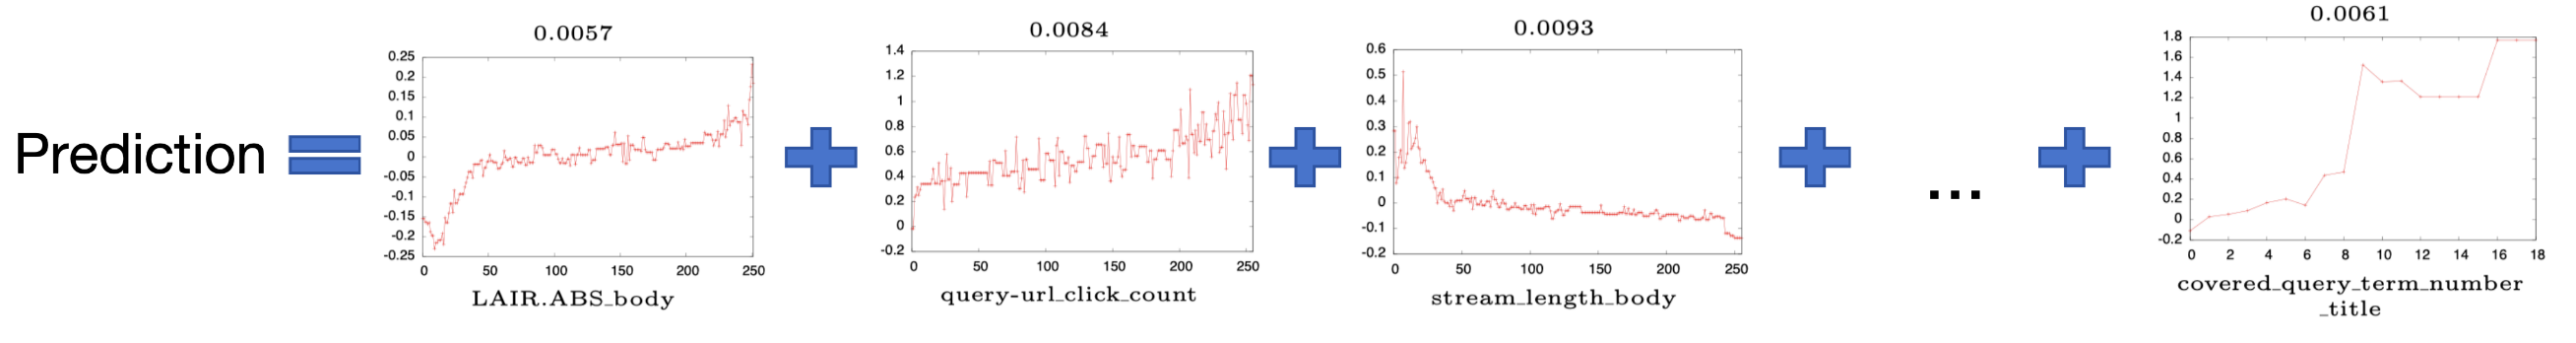
\includegraphics[width=1.3\linewidth]{figure/ebm_prediction.png}
    \label{fig:Intelligible ebm_prediction}
\end{figure}
\end{frame}

\begin{frame}{Intelligible GAM - Novelty and Extension}
\begin{itemize}
    \item In each boosting step, use a bagging tree limited in size (2-4 leaves) \begin{itemize}
        \item High accuracy, low variance, prevent overfitting
        \item Provides discrete shape functions
        \item Captures missing information in spline plots
        \item High intelligibility
    \end{itemize}
    \item Not as accurate as unrestricted full complexity model
    \item In the next step: \citebutton{Lou et al. 2013}{https://www.cs.cornell.edu/~yinlou/papers/lou-kdd13.pdf}
    \begin{itemize}
        \item Add pairwise feature interaction terms to the model
        \item Replace the 2-4 regions of small tree
        \item By a dynamic programming algorithm called FAST
    \end{itemize}
\end{itemize}
\end{frame}

\begin{frame}{Accurate GAM plus Pairwise Interactions}
\textbf{Generalized Additive Models plus Interactions}: $$g(\E (y \mid \xv)) = \theta_0 + \sum f_i(x_i) + \sum f_{ij}(x_i,x_j)\quad for\quad i,j=1,\cdots,p,\quad i\neq j$$
\begin{itemize}
    \item $O(p^2)$: a large number of pairwise interactions if $p$ is big\\
    $\leadsto$ Select only a small number of the most important interactions
    \item Intuitively, significant reduction in RSS $\to$ Strong pair interaction
    \item \textbf{FAST} algorithm does quick ranking without fully building every interaction function
\end{itemize}
\end{frame}

\begin{frame}{FAST feature interaction detection - PART I}

\begin{columns}[T, totalwidth=\textwidth]
\begin{column}{0.5\textwidth}
\begin{figure}
    \centering
    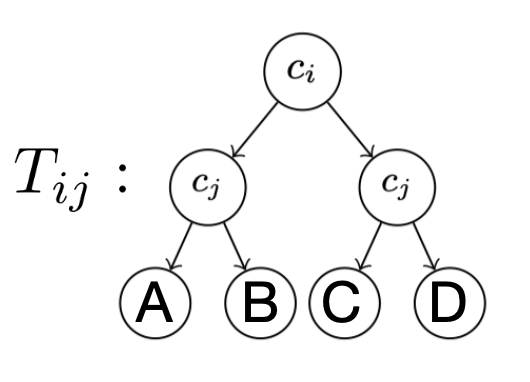
\includegraphics[width=0.6\linewidth]
    {figure/T_ij.png}
    \label{fig:tree-like predictor}
\end{figure}
\begin{figure}
    \centering
    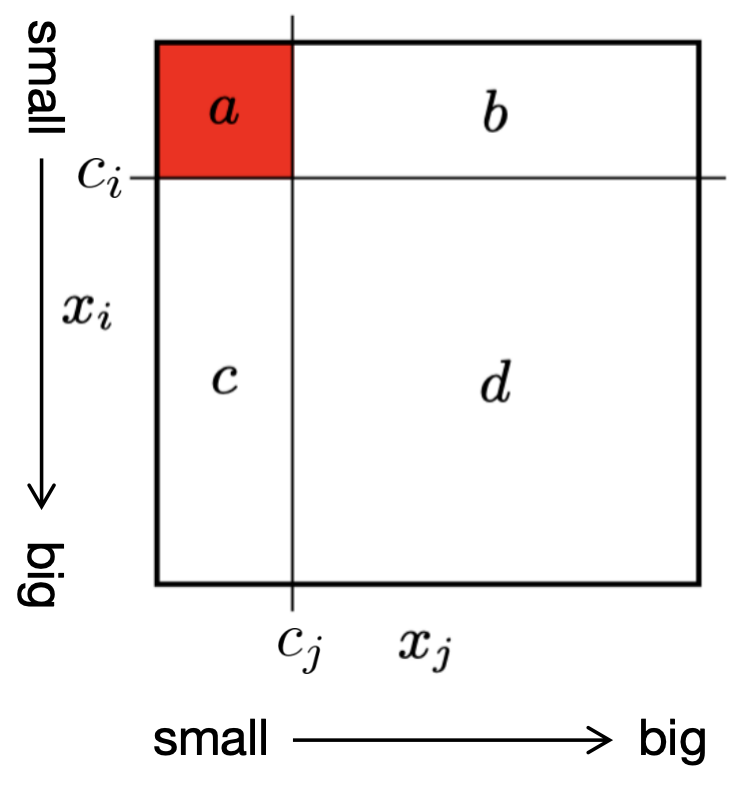
\includegraphics[width=0.65\linewidth]
    {figure/FAST1.png}
    \label{fig:FAST1}
\end{figure}
\end{column}
\hfill
\centering
\begin{column}{0.6\textwidth}
\begin{itemize}
    \item $T_{ij}$: A tree-like interaction predictor with 4 leaves for each pair of features
    \item $c_i$, $c_j$: One cut (grid point) on the \textbf{sorted} values of feature $x_i$ and $x_j$, respectively
    \item $A$, $B$, $C$, $D$: Notation for 4 leaf regions
    \item \textbf{Idea}: Search for all possible $(c_i, c_j)$ and pick the best $T_{ij}$ with the lowest RSS
    \item Prediction value on region r, $r\in\{A, B, C, D\}$:
    $$\hat{y}_r=T_{ij}.r=\frac{1}{\vert r\vert}\sum_{(\mathbf{x},y)\in r}y=\frac{\text{Sum of targets in }r}{\text{Sum of counts in }r}$$
    \item $\text{RSS}=\sum_{k=1}^N(y_k-T_{ij}(\mathbf{x}_k))^2$ \\
    \qquad\;$=\sum_{k=1}^Ny_k^2-2\sum_r\left(\hat{y}_r\cdot\sum_{(\mathbf{x},y)\in r}y\right)$\\
    \qquad\;\;\;\;$+\sum_r\hat{y}_r^2\cdot\vert r\vert$
\end{itemize}
\end{column}
\end{columns}

\end{frame}

\begin{frame}{FAST feature interaction detection - PART II}

\begin{columns}[T, totalwidth=\textwidth]
\begin{column}{0.5\textwidth}
\begin{itemize}
\item How to quickly get sum of targets and sum of counts for all possible cuts?\\
    $\leadsto$ Use \textbf{marginal cumulative histograms} (CH)
\end{itemize}
\begin{figure}
    \centering
    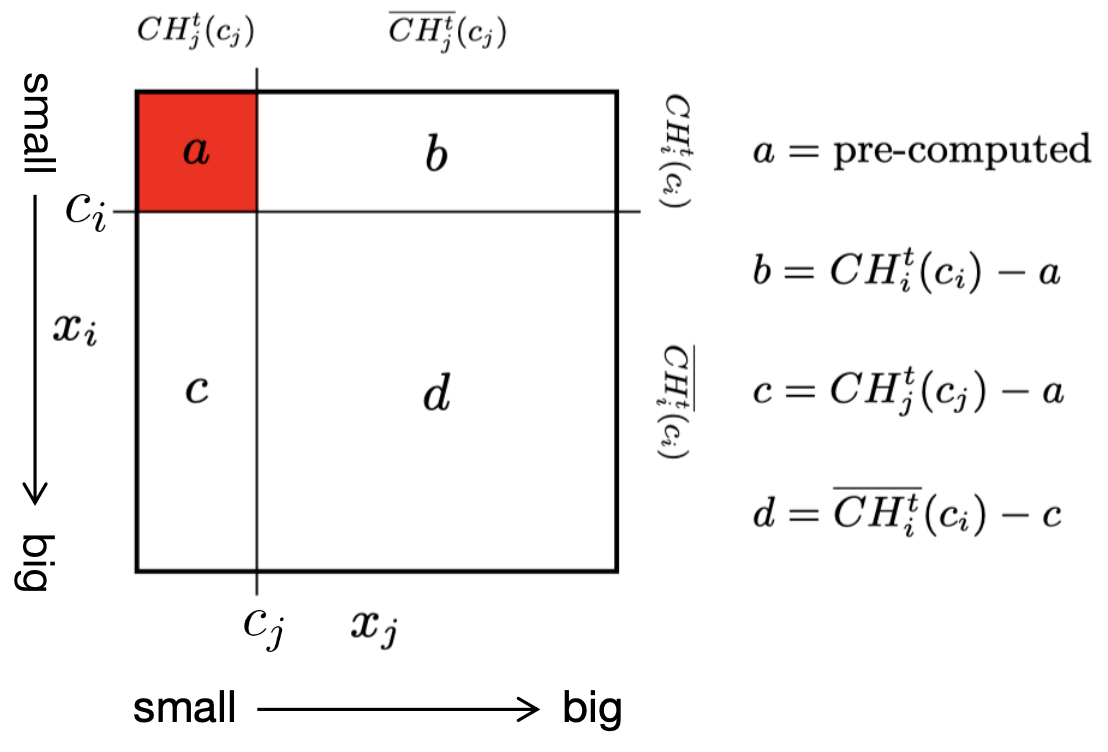
\includegraphics[width=\linewidth]
    {figure/FAST.png}
    \\An illustration for computing sum of targets for each quadrant
    \label{fig:FAST2}
\end{figure}
\end{column}
\hfill
\centering
\begin{column}{0.6\textwidth}
\begin{itemize}
    \item For example:\\
    $CH_j^t(c_j)$: cumulative sum of targets for data points with $x_j\leq c_j$;\\
    $\overline{CH_j^t }(c_j)$: cumulative sum of targets for data points with $x_j>c_j$
    \item Create \textbf{two lookup tables} to store values for every $(c_i, c_j)$, :\\
    1. Compute the cumulative sum of targets in four regions, and store the values in the \textbf{table of targets} $L^t(c_i,c_j)=[a,b,c,d]$\\
    2. Compute the cumulative sum of counts in four regions, and store the values in the \textbf{table of counts} $L^w(c_i,c_j)=[a,b,c,d]$
    \item Given any $(c_i, c_j)$, values of $(b,c,d)$ can be easily derived with known $\color{red}a$\\
    $\leadsto$Construct lookup tables using dynamic programming
\end{itemize}
\end{column}
\end{columns}

\end{frame}

\begin{frame}{FAST feature interaction detection - PART III}

\begin{itemize}
    \item For $x_i$ with $d_i$ possible values and $x_j$ with $d_j$ possible values:\\
    $\leadsto$ compute and store $d_id_j$ records of $[a,b,c,d]$ in both table of targets and table of counts
    \item For each pair of $(x_i,x_j)$, calculate RSS for each possible $(c_i, c_j)$ and pick the best $T_{ij}$ with the lowest RSS [Note: $\hat{y}_A$ can be simply calculated as $L^t(c_i,c_j).a/L^w(c_i,c_j).a$]
\end{itemize}
\[
\text{\qquad$d_id_j$ possible $(c_i, c_j)$}
\left\{
\begin{array}{@{}l@{\quad}l@{\quad}l@{\quad}l@{\quad}l}
    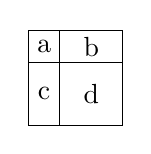
\begin{tikzpicture}[baseline=(current bounding box.center)]
        \draw (0,0) rectangle (1.2,1.2);
        \draw (0.4,0) -- (0.4,1.2); 
        \draw (0,0.8) -- (1.2,0.8); 
        \node at (0.2,0.4) {c};
        \node at (0.8,0.4) {d};
        \node at (0.2,1) {a};
        \node at (0.8,1) {b};
    \end{tikzpicture} & \text{$\Rightarrow$} & 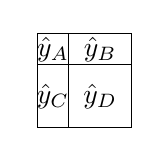
\begin{tikzpicture}[baseline=(current bounding box.center)]
        \draw (0,0) rectangle (1.2,1.2);
        \draw (0.4,0) -- (0.4,1.2); 
        \draw (0,0.8) -- (1.2,0.8); 
        \node at (0.2,0.4) {$\hat{y}_C$};
        \node at (0.8,0.4) {$\hat{y}_D$};
        \node at (0.2,1) {$\hat{y}_A$};
        \node at (0.8,1) {$\hat{y}_B$};
    \end{tikzpicture} & \text{$\Rightarrow$} & \text{$RSS_1$}\\[0.7cm] 
    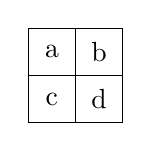
\begin{tikzpicture}[baseline=(current bounding box.center)]
        \draw (0,0) rectangle (1.2,1.2);
        \draw (0.6,0) -- (0.6,1.2); 
        \draw (0,0.6) -- (1.2,0.6); 
        \node at (0.3,0.3) {c};
        \node at (0.9,0.3) {d};
        \node at (0.3,0.9) {a};
        \node at (0.9,0.9) {b};
    \end{tikzpicture} & \text{$\Rightarrow$} & 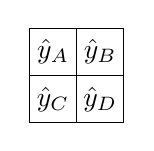
\begin{tikzpicture}[baseline=(current bounding box.center)]
        \draw (0,0) rectangle (1.2,1.2);
        \draw (0.6,0) -- (0.6,1.2); 
        \draw (0,0.6) -- (1.2,0.6); 
        \node at (0.3,0.3) {$\hat{y}_C$};
        \node at (0.9,0.3) {$\hat{y}_D$};
        \node at (0.3,0.9) {$\hat{y}_A$};
        \node at (0.9,0.9) {$\hat{y}_B$};
    \end{tikzpicture} & \text{$\Rightarrow$} & \text{$RSS_2$}\\[0.7cm] 
    \makebox[1cm][c]{\vdots} & & \makebox[1cm][c]{\vdots} & & \makebox[1cm][c]{\vdots}\\[0.3cm]
    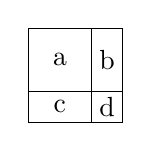
\begin{tikzpicture}[baseline=(current bounding box.center)]
        \draw (0,0) rectangle (1.2,1.2);
        \draw (0.8,0) -- (0.8,1.2); 
        \draw (0,0.4) -- (1.2,0.4); 
        \node at (0.4,0.2) {c};
        \node at (1,0.2) {d};
        \node at (0.4,0.8) {a};
        \node at (1,0.8) {b};
    \end{tikzpicture} & \text{$\Rightarrow$} & 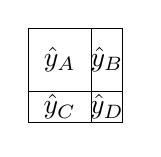
\begin{tikzpicture}[baseline=(current bounding box.center)]
        \draw (0,0) rectangle (1.2,1.2);
        \draw (0.8,0) -- (0.8,1.2); 
        \draw (0,0.4) -- (1.2,0.4); 
        \node at (0.4,0.2) {$\hat{y}_C$};
        \node at (1,0.2) {$\hat{y}_D$};
        \node at (0.4,0.8) {$\hat{y}_A$};
        \node at (1,0.8) {$\hat{y}_B$};
    \end{tikzpicture} & \text{$\Rightarrow$} & \text{$RSS_{d_id_j}$}\\ 
\end{array}
\right\}
\text{\parbox[t]{6cm}{select the lowest RSS and assign it as the weight for $(x_i, x_j)$ to measure the strength of interaction}}
\]
\end{frame}

\begin{frame}{FAST feature interaction detection - PART IV}
\begin{itemize}
    \item Complexity analysis: \\
    Computing cumulative histograms: $O(N)$ ($N$: number of observations)\\
    Constructing matrices of sum values: $O(N+d_id_j)$\\
    $\leadsto$ Complexity per pair: $O(N+d_id_j)$ 
    \item Discretize continuous feature values in $b$ bins ($b\leq256$)\\
    $\leadsto O(N+b^2)$ per pair\\
    $\leadsto$ Choose optimal number of bins $b$ w.r.t. bias-variance trade-off
    \item Quick ranking and select top K pairs
\end{itemize}
\end{frame}

\begin{frame}{Accurate GAM - Two-stage Construction}
\begin{enumerate}
    \item Fit main effects
    \begin{itemize}
        \item Fit model only using univariate terms
        \item Fix the main effects model
    \end{itemize}
    \item Fit pairwise residual of main effects model to original targets
    \begin{itemize}
        \item Use FAST to sort through $O(p^2)$ pairs
        \item User selects number $K$ of pairs to be added
        \item Run boosting algorithm to fit $K$ pairs
        \item Final model = $p$ mains + $K$ pairs
    \end{itemize}
\end{enumerate}
\end{frame}

\begin{frame}{Accurate GAM - 2. Stage Algorithm Sketch}
\begin{figure}
    \centering
    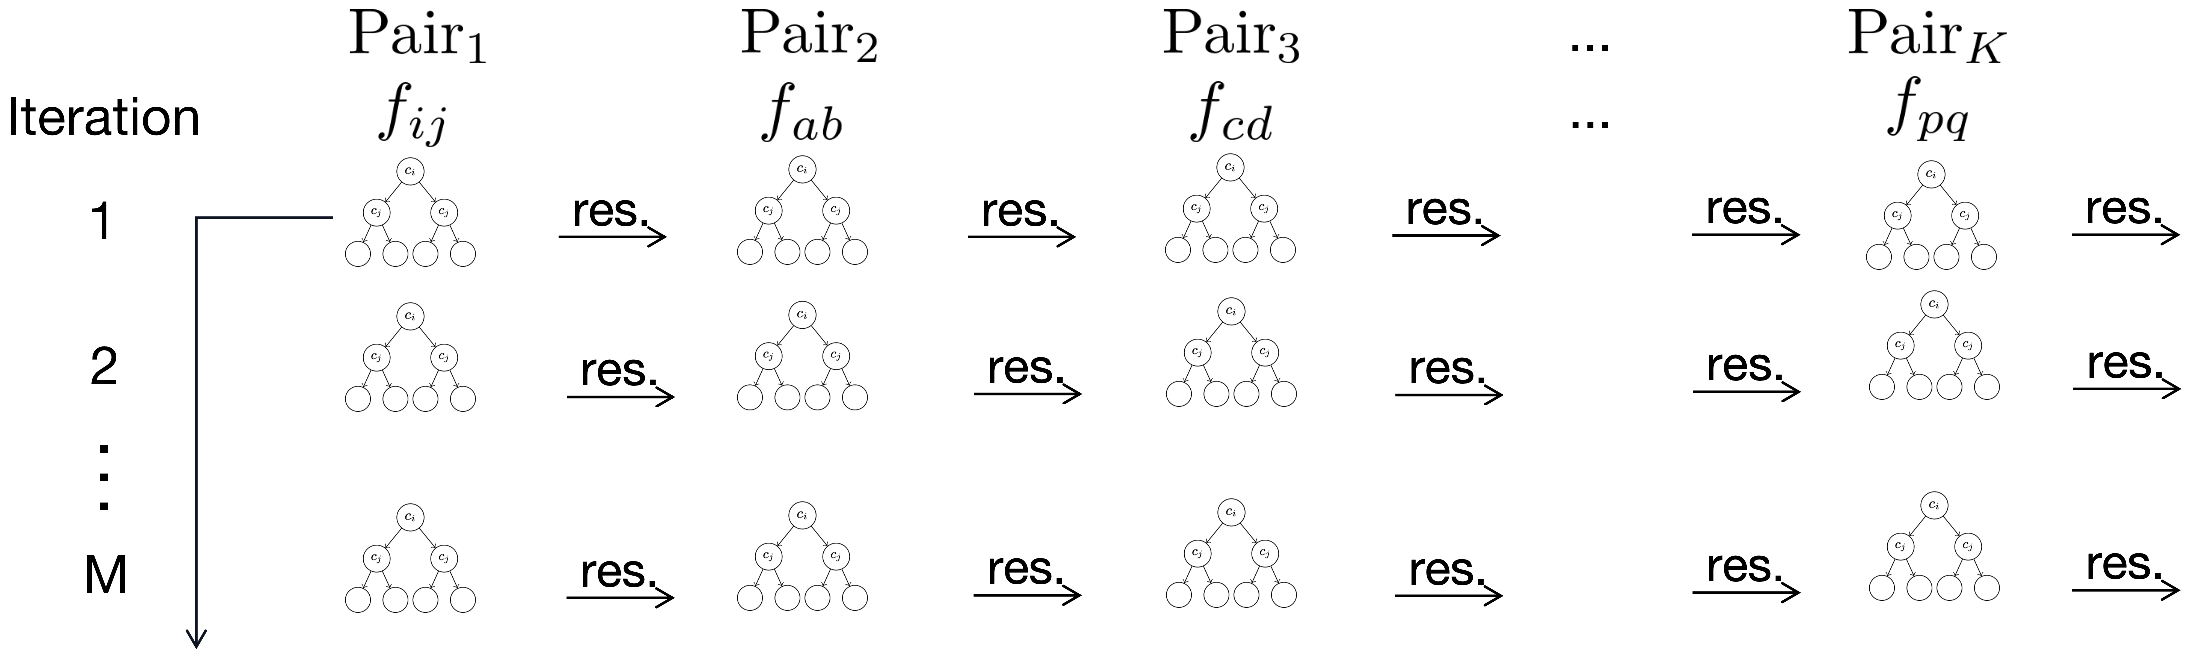
\includegraphics[width=1\linewidth]{figure/GA2M_Step1.png}
    \label{fig:GA2M_Step1}
\end{figure}
\begin{columns}[T, totalwidth=\textwidth]
    \begin{column}{0.4\textwidth} 
        \begin{figure}
            \vspace{-1.35cm} 
            \hspace{-0.8cm} 
            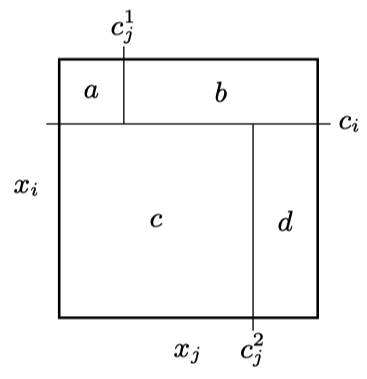
\includegraphics[width=0.8\linewidth]{figure/GA2M_Step0.png}
            \label{fig:GA2M_predictor}
        \end{figure}
    \end{column}
    \hfill
    \begin{column}{0.7\textwidth}
        \begin{itemize}
            \setlength{\leftskip}{-0.7cm}
            \vspace{-0.8cm}
            \item To model the pairwise interactions effectively and efficiently\\
            $\leadsto$Replace the shallow tree ensembles used in Intelligible GAM with a tree-like predictor (similar to FAST)
            \item 3 cuts instead of 2 cuts
            \item Re-use the stored values in the lookup tables for sum of targets and sum of counts from FAST
            \item Greedy search for the best combination of cuts (lowest RSS)
        \end{itemize}
    \end{column}
\end{columns}

\end{frame}

\begin{frame}{Accurate GAM - Prediction}
\begin{itemize}
    \item Output: $M$ predictors which were only trained on $\text{Pair}_1$ \\
    \qquad\;\; + $M$ predictors which were only trained on $\text{Pair}_2$ \\
    \qquad\;\; $\cdots$ \\
    \qquad\;\; + $M$ predictors which were only trained on $\text{Pair}_K$
    \item Summarize the weighted predictions of $M$ models in a 3D heatmap
    \item The dimension of color represents the contribution of pairwise feature values to the prediction
    \item Generate a 3D heatmap for each pair of features
\end{itemize}

\begin{figure}    
    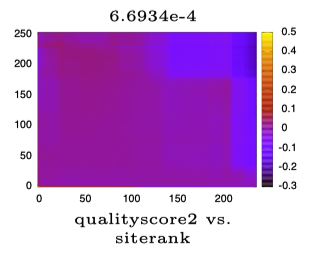
\includegraphics[width=0.4\linewidth]
    {figure/3D Heatmap.png}
    \label{fig:3D Heatmap}
\end{figure}

\end{frame}

\begin{frame}{EBM - Final Model}
\begin{figure}    
    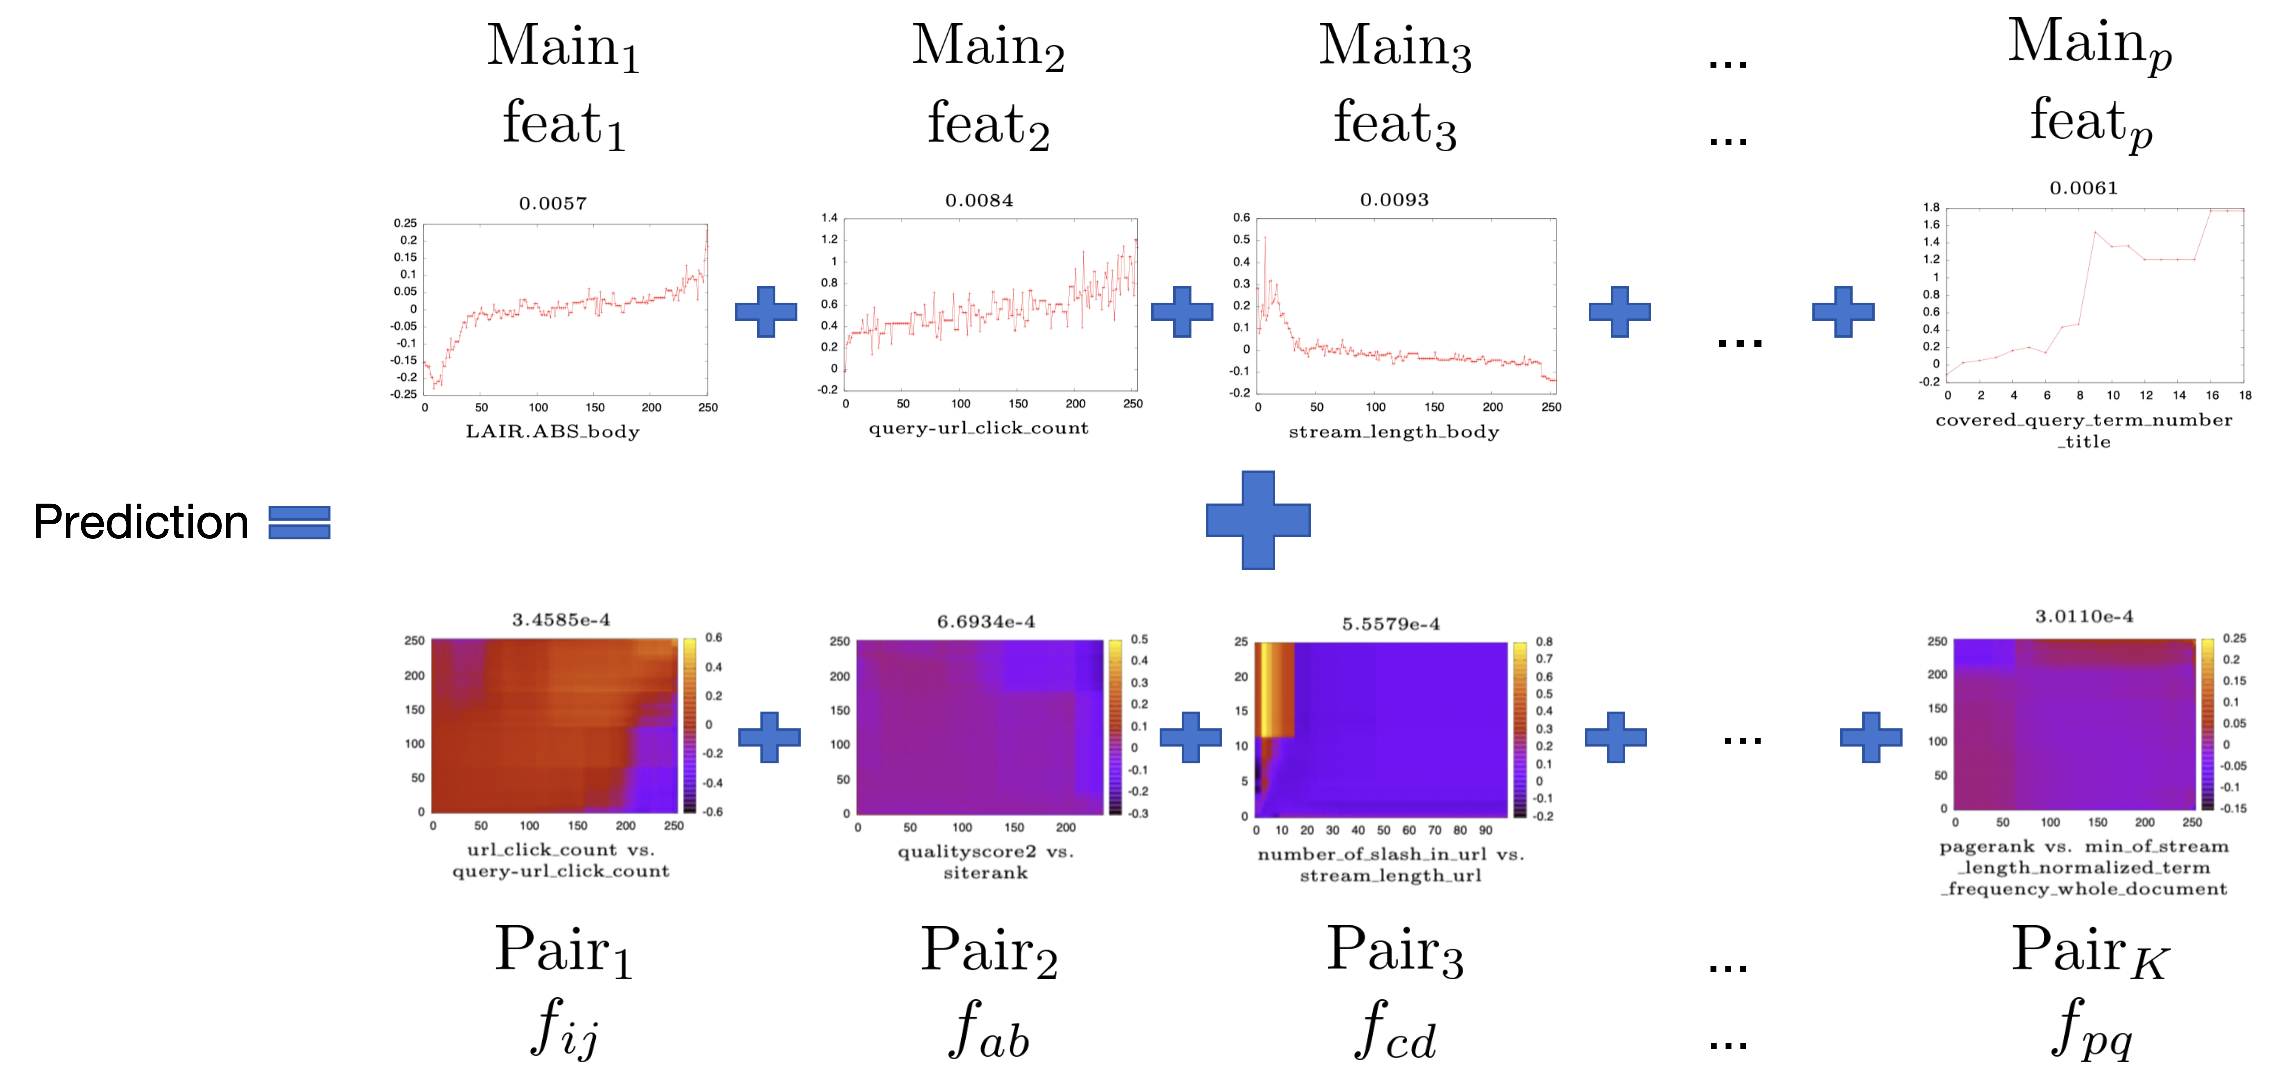
\includegraphics[width=1\linewidth]
    {figure/final_ebm.png}
    \label{fig:final_ebm}
\end{figure}
\end{frame}

\end{document}